\documentclass{llncs}
\usepackage{graphicx}
\graphicspath{ {images/} }
\bibliographystyle{splncs}

\title{\textbf{Random Forest vs Logistic Regression for Binary Classification}}
\author{Kaitlin Kirasich, Trace Smith, and Bivin Sadler, PhD$^1$}
\institute{Master of Science in Data Science \\ Southern Methodist University \\ Dallas, Texas USA \\
\email{kkirasich@.smu.edu,traces@smu.edu,bsadler@smu.edu}}

\begin{document}
\maketitle

\begin{abstract} 
Selecting a learning algorithm to implement for a particular application on the basis of performance still remains an ad-hoc process using fundamental benchmarks such as evaluating a classifier’s overall loss function, area under the curve (AUC) score, specificity, and sensitivity values. In this paper we address the difficulty of model selection by evaluating the overall classification performance between random forest and logistic regression for datasets comprised of various underlying structures. We developed a model evaluation tool capable of simulating classifier models for a range of dataset characteristics and performance metrics such as true positive rate, false positive rate, and accuracy under specific conditions. We found that when increasing the variance in the explanatory and noise variables, logistic regression consistently performed with a higher overall accuracy as compared to random forest. However, the true positive rate for random forest was higher than logistic regression and yielded a higher false positive rate for dataset with increasing noise variables. In all simulated case studies, we consistently found that the false positive rate for random forest with 100 trees was statistically different than logistic regression. 

\end{abstract}


\section{Introduction}

\noindent 
Datasets are composed of various dimensions and underlying structures. We have discovered the relative performance of machine learning algorithms with varying data characteristics is not well documented. Depending on whether binary or multiple class labels in a 'n' dimensional space are linearly separable or not, the overall model performance weights heavily on the algorithm selected for implementation. Complex models like decision trees or other non-parametric algorithms can have decision boundaries with high variance and low bias which can often lead to overfitting if not properly tuned. The idea of overfitting is the result of a model with a high classification score on a training set while generalizing poorly on an out of sample datasets. On the other hand, parametric based models like logistic regression are less complex, resulting in a linear decision boundary that can have a higher bias. This can translate to underfitting as the model fails to adequately learn patterns in the data for accurate predictions if not tuned properly. Balancing the bias vs variance trade-off is driven in large part by the simplicity or complexity of the data structure being modeled. 

\noindent 
Depending on the structure of the dataset being modeled, deciphering which algorithm to deploy in order to achieve the highest performance scores still remains an ad-hoc process. This prompts the questions, under what circumstances does one model begin to outperform another model? For instance, when increasing the number of noise and explanatory variables in a dataset, at what point does the relative model performance begin to deviate between models? To answer these questions, our work consisted of building an analytical tool that simulates various data complexities and directly observe the classification performance of each model by averaging metrics for 1000 random generations of assorted multivariate datasets. Classification is a form of supervised learning in which an algorithm aims to classify which category or categories an input belongs to. Supervised learning can be described as taking an input vector comprised of 'n' features and mapping it to an associated target value or class label. The term 'supervised' originated from the concept that the training and testing datasets contain a response label and the algorithm observes the input vector and attempts to learn a probability distribution to predict 'y' given 'x' \cite{goodfellow}. To compare model performance, classification metrics such as accuracy, area under the curve, true positive rate, false positive rate, and precision were analyzed. In order to provide statistical quantification as to whether a difference in model performance is conclusive enough to state the difference is significant or if the observed difference is by random chance, a pairwise two-sample t-test is also conducted at the end of each simulation case study 

\noindent 
For the sake of interoperability and computation time for model training, we considered one parametric and non-parametric for binary classification, logistic regression and random forest, respectively. Both classifiers have been widely implemented in various domains and their successes have been well documented. However, the particular characteristics of a dataset that make one model outperform the other is unknown as most published work compares overall performance between the two models for a single dataset. Classifiers like the ones presented in this work, logistic regression and random forest, learns a series of weights or parameters that determine how the input feature vector affects the prediction. The objective of the algorithm is to minimize the error or loss between the ground truth and predicted value in order to precisely classify the input to the associated label.


\section{Background}
\noindent 

A dataset is a collection of an arbitrary number of observations and descriptive features which can be numerical, categorical or a combination of the two. Characteristics of a dataset can be comprised of missing values, outlier, highly correlated variables, concave or convex shapes, or subsets of the data that can be represented as clusters. Complex datasets that are not linearly separable, or in other words, where a linear hyperplane splits the data into two halves such that the model poorly predicts the class label of the respected observation (Figure~\ref{fig:boundary1}). One approach to inferring underlying complexities of high-dimensional dataset is Topological Data Analysis (TDA). TDA is an evolving method that utilizes topological and geometric tools to identify relevant features in the data. TDA can be described as method that helps identify structures in noisy and incomplete datasets like clusters or other hidden shapes that can provide a more accurate representation of the dataset \cite{chazal}. Models can then be trained on the new representation of the data that has been reconstructed, which has shown promising results. While TDA looks at the proximity of data points and connectivity that can be mapped to a 1-dimensional plane for representing the shape of the data \cite{munch}, our analysis is aimed at creating various complexities in the data and evaluating model performance on the raw structure in a multidimensional space. For instance, altering the variance in the explanatory and noise variables, changing the number of observations, and varying the number of continuous features included in a multivariate dataset was considered. Investigation into why models like logistic regression or random forest perform differently for simple and complex data characteristics was the motivation behind this work.

\noindent 
The data examined in this work is only for continuous variables that have a Gaussian distribution. However, more complex structures can exist like the toy dataset shown below in Figure~\ref{fig:boundary1} and Figure~\ref{fig:boundary2} which consists of concave and convex shape. As illustrated in these figures, both random forest and logistic regression nearly establishes an identical decision boundary for the left-hand side dataset. Alternatively, logistic regression underperforms random forest and yields a higher misclassification rate, which raises a profound question as to which data characteristics constitutes one model achieving an overall better classification score. It should be noted this work only investigates random forest and logistic regression, however generalization of the current application can be adapted to other linear and nonlinear models. Performance of machine learning classifiers can yield varying results depending on the shape and structure of the data.

\begin{figure}
\centering
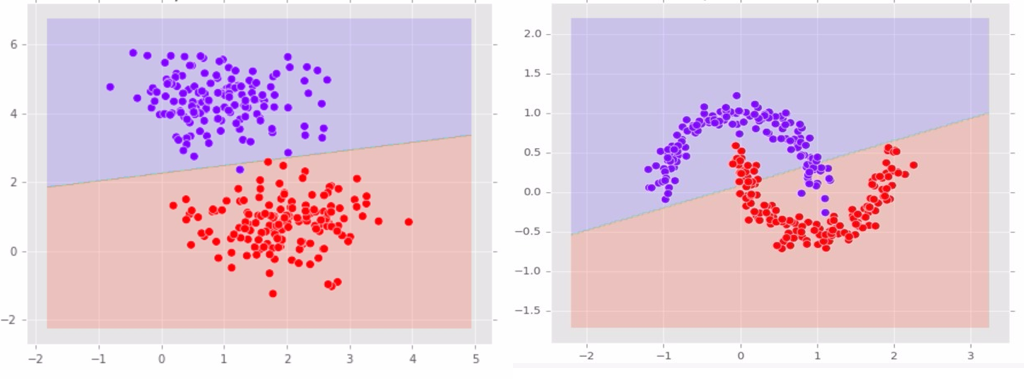
\includegraphics[width=0.9\textwidth]{decisionboundary.png}
\caption{Logistic Regression and Random Forest}
\label{fig:boundary1}
\end{figure}

\begin{figure}
\centering
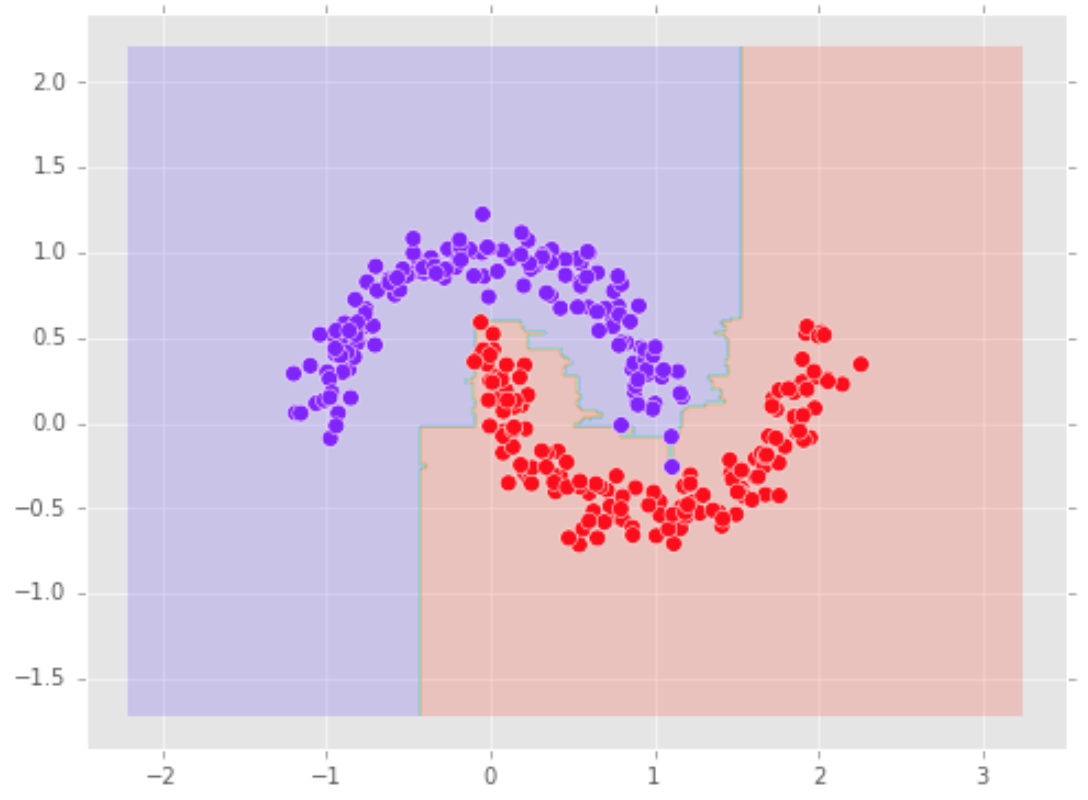
\includegraphics[width=0.9\textwidth]{decisionboundary2.png}
\caption{Random Forest (n-Trees = 100) Decision Boundary}
\label{fig:boundary2}
\end{figure}

\noindent 
Numerous studies have been published that compare random forest and logistic regression algorithms however, most research experiments consisted of either a single dataset or multiple datasets from the same source. In these scenarios, sometimes logistic regression performed better while in other cases random forest performed better. For example, one experiment used several neuropsychological tests to predict dementia stated that with respect to specificity and overall classification accuracy, random forests and linear discriminant analysis rank first among all the classifiers including logistic regression (Guerreiro, 2011). In this case study, data for 921 elderly non-demented patients with complaints that were referred for neuropsychological evaluation at three different institutions between from 1999 to 2007 was collected. At the follow-up of each evaluation, subjects were either classified as being diagnosed with dementia or not. Metrics such as sensitivity, specificity, ROC, and accuracy were evaluated using five fold cross validation. Results indicated Random Forests and Linear Discriminant Analysis proved to have the highest accuracy, sensitivity, specificity compared to other models. Median overal accuracy and ROC for Random Forest is 0.73, respectively.   

\noindent 
Contrastingly, another publication analyzed Twitter tweets surrounding the 2016 United States election. A data set of 850 observations and 299 features extracted from tweets obtained during the election period were utilized to classify voter sentiment and whether a tweet was either political or non-political. In addition to analyzing feature importance, random forest yielded the highest overall accuracy score of 95\%. Several cases were considered, such as including all of the explanatory variables in the model and performing dimensionality reduction by applying Principal Component Analysis. In all cases, random forest consistently produced higher f1 and accuracy scores compared to logistic regression and support vector machines \cite{erdem}. 

\noindent 
Random forest and logistic regression have been compared in numerous studies on specific datasets and have both yielded varying performances. In the work presented by Ruiz-Gazen et al on classifying satellite measurements of cloud systems as either convective or non convective systems \cite{ruiz}. With 41 numerical variables built from satellite measurements to train models on, the class labels were heavily skewed with only less than five percent of the labels being non-convective. The overall model results indicate virtually identical performance, however the authors recommeded using logistic regression due to the interpretation of parameter estimates of the explanatory varibles in addition to quicker computation time to train models \cite{ruiz}. The type of data and data sources used in the studies above are drastically different from each other and each algorithm performs differently due to the type of data it was utilizing to train each classifier. This analysis aims to provide a method of evaluating random forest and logistic regression models by simulating a variety of data characteristics and then evaluate which model yielded better performance under certain conditions.

\noindent 
In Data Science, there is also a "No-free-lunch" theorem for supervised algorithms which says that all algorithms that search for an extremum of a cost function perform exactly the same when averaged over all possible cost functions \cite{wolper}.  Many researchers have set out to find one algorithm that performs better than another.  However, the no free lunch theorem tells us that if one algorithm outperforms another in one metric, it will lose in another metric. Wolpert found that in a noise-free scenario where the loss function is the misclassification rate, there are no distinctions between learning algorithms when averaged over all possible cost functions.  The research shows that a better performance over one class of problems is equivalently paid for in performance of another class of problems.  "In particular, if algorithm A outperforms algorithm B on some cost functions, then loosely speaking there must exist exactly as many other functions where B outperforms A."\cite{wolper}. One of the motivations behind this work with the no free lunch theorem is to study how random forest and logistic regression perform under various data complexities by using different performance metrics like AUC, ROC, true prositive rate, and false positive rates.

\section{Machine Learning Algorithms}

\noindent 
The two machine learning algorithms studied in this work consist of random forest and logistic regression. Both models have been widely implemented successfully in various disciplines for classification and regression purposes \cite{couronne}. The functionality of logistic regression, a parameter based model, and random forest, a non-parametric model, are summarized in the following section. 

\subsection{Random Forest}

\noindent 
Random forest is an ensemble-based learning algorithm which is comprised of n collections of de-correlated decision trees (Hastie, 2009). It is built off the idea of bootstrap aggregation, which is a method for resampling with replacement in order to reduce variance. Random Forest uses multiple trees to average (regression) or compute majority votes (classification) in the terminal leaf nodes when making a prediction. Built off the idea of decision trees, random forest models have resulted in significant improvements in prediction accuracy as compared to a single tree by growing 'n' number of trees; each tree in the training set is sampled randomly without replacement \cite{breiman}. Decision trees consist simply of a tree-like structure where the top node is considered the root of the tree that is recursively split at a series of decision nodes from the root until the terminal node or decision node is reached. 

\noindent 
As illustrated in the tree structure (Figure~\ref{fig:tree}), the decision tree algorithm is a top down greedy approach that partitions the dataset into smaller subsets. The result is a tree with a series of decision nodes until the leaf nodes are reached, which is used to make a prediction. The predictor variable that yields the highest information gain is the root node. The leaf nodes is represented as a prediction, and in this case, classifying either 1 or 0. Decision trees can handle both categorical and numerical data. First, in order to determine the information gain which is based on the entropy after splitting on an attribute, entropy is computed. Information gain is based on the principles from information theory that uses entropy to compute impurity of datasets. Entropy measures the homogeneity of the subset data; if entropy equals one then the class labels are equally divided while an entropy of zero means the sample is completely homogeneous. 


\begin{figure}
\centering
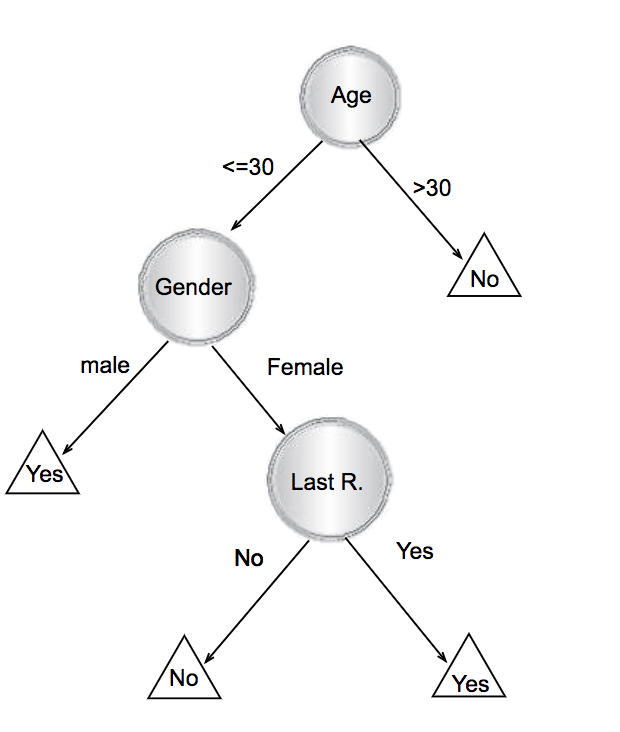
\includegraphics[width=0.5\textwidth]{decisiontree.png}
\caption{Example of Decision Tree (Lior Rokach et al)}
\label{fig:tree}
\end{figure}


At each decision node, the entropy for each attribute in the model is computed prior to making a split. 


\begin{equation}
Entropy = -p\log_{2}(p) - q\log_{2}(q)
\end{equation}


\noindent 
Advantages of using a tree-like learning algorithm allow for training models on large datasets in addition to quantitative and qualitative input variables. Additionally, tree-based models can be immune to redundant variables or variables with high correlation which may lead to overfitting in other learning algorithms. Trees also have very few parameters to tune for when training the model and performs relatively well with outliers or missing values in a dataset. However, trees are prone to poor prediction performance; decision trees themselves are prone to overfitting noise in a training set which ultimately leads to results with high variance. In other words, this means the model could accurately predict the same data it was trained on but may not possess the same performance on datasets without the similar patterns and variations in the training set. Even fully grown decision trees are notorious for overfitting and do not generalize well to unseen data; random forest solves the overfitting conundrum by using a combination or "ensemble" of decision trees where the values in the tree are a random, independent, sample. 


\noindent 
Randomly sampling without replacement is known as bagging and this results in a different tree being generated to train on; averaging the results from the 'n' number of trees will result in decreasing the variance and establishing a smoother decision boundary \cite{hastie}. For instance, while using random forest for classification, each tree will give an estimate of the probability of the class label, the probabilities will be averaged over the 'n' trees and the highest yields the predicted class label (Figure~\ref{fig:rftree}). In addition to bagging or bootstrap aggregation, in order to further reduces the variance in the decision boundary further, the trees must be completely uncorrelated and the method of bootstrapping alone is not enough. Breiman introduced the idea of randomly sampling 'm' number of features at each decision split in the tree as a way to de-correlate the trees in the random forest algorithm \cite{breiman}.  


\begin{figure}
\centering
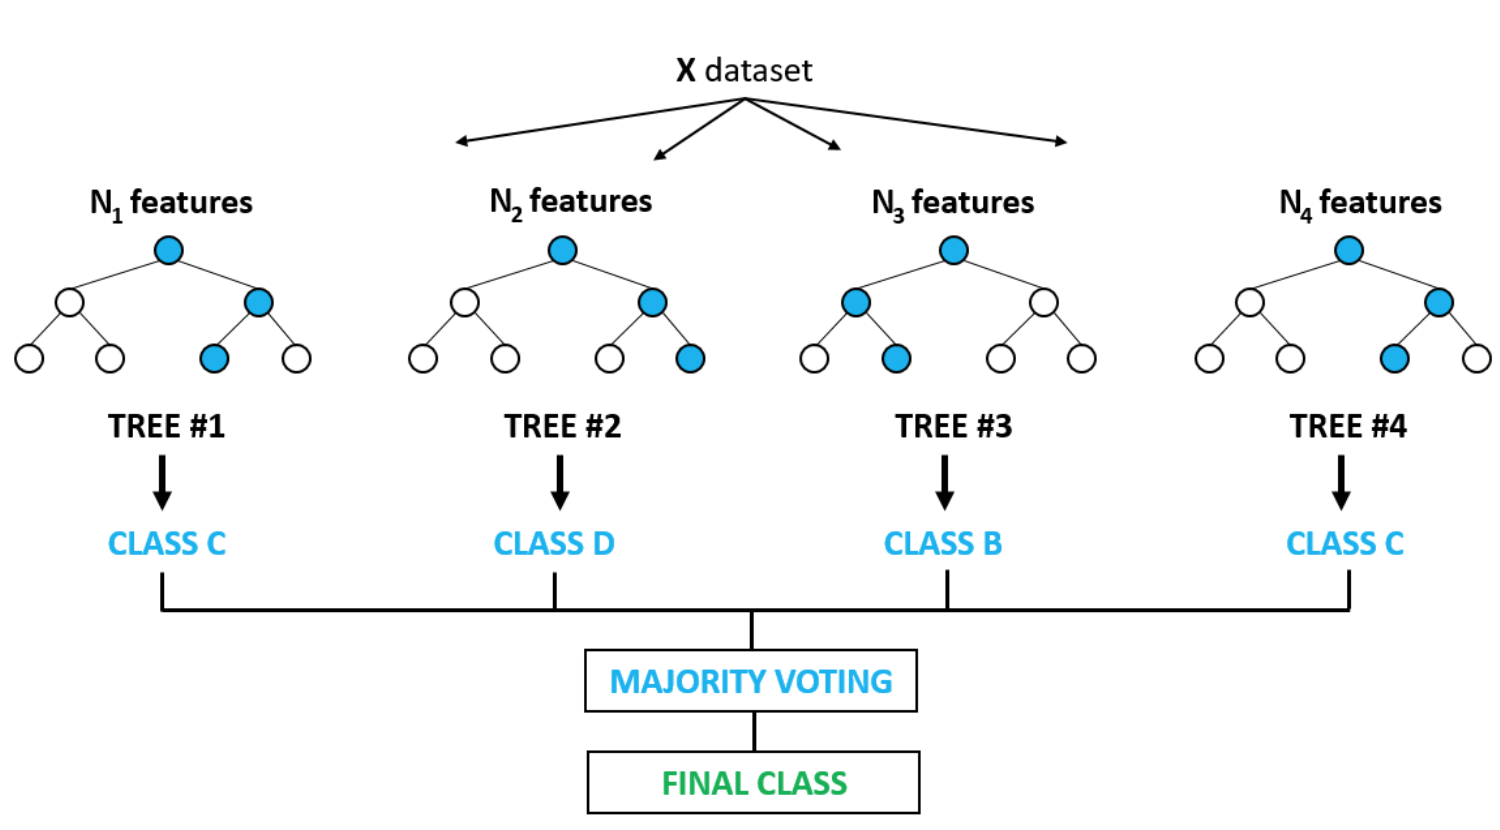
\includegraphics[width=0.90\textwidth]{randomforest.png}
\caption{Example of Decision Tree (Balazs Holczer)}
\label{fig:rftree}
\end{figure}

\subsection{Logistic Regression}

\noindent 
Linear models are composed of one or multiple independent variables that describes a relationship to a dependent response variable. Mapping qualitative or quantitative input features to a target variable that is attempted to being predicted such as financial, biological, or sociological data is known as supervised learning in machine learning terminology if the labels are known.  One of the most common utilized linear statistical models for discriminant analysis is logistic regression.

\begin{equation}
\pi_{i} = \beta_{0} + \beta_{1}X_{1} + .....\beta_{n}X_{n}
\end{equation}


\noindent 
Simplicity and interoperability of logistic regression can occasionally lead to outperforming other sophisticated nonlinear models such as ensemble learners or support vector machines. However, in the event the response variable is drawn from a small sample size, then logistic regression models become insufficient and performs poorly for binary responses A number of learning algorithms could be applied to modeling binary classification data types, however the focal point of this work is to examine one linear model, logistic regression. 
 
 
 \noindent 
In the case of logistic regression, the response variavle is response varialbe is quantitative. For logistic regression, the response variable is the posterior probability of being classified in the ith group of a binary or multi-class response \cite{hastie}. Logistic regression makes several assumptions such as independence, responses (logits) at every level of a subpopulation of the explanatory variable are normally distributed, and constant variance between the responses and all values of the explanatory variable. Intuitively, a transformation to the response variable is applied to yield a continuous probability distribution over the output classes bounded between 0 and 1; this transformation is called to “logistic” or “sigmoid” function where ‘z’ corresponds to log odds divided by the logit \cite{ng}. The parameter estimates inform whether there is an increase or decrease in the predicted log odds of the response variable that would be predicted by one unit increase or decrease in one of the explanatory variables (e.g. x1), while holding all other explanatory variables constant.

\begin{equation}
\sigma(Z) = \frac{1}{1+\exp^{-z}}
\end{equation}


\begin{figure}
\centering
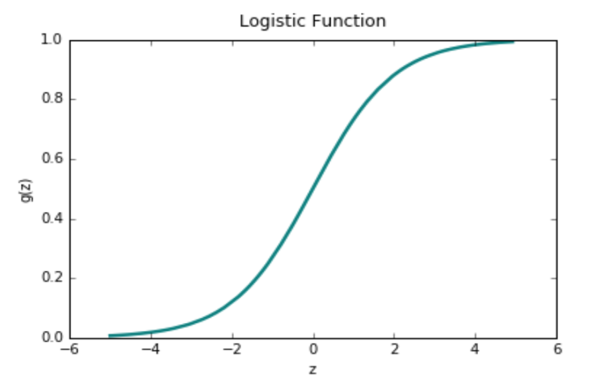
\includegraphics[scale=1.0]{sigmoid.png}
\caption{Logistic Function}
\end{figure}


\noindent 
For a binary response, the logistic regression model can be expressed by summing over the linear combinations of input features and a corresponding weight plus a bias term for each instance as shown below in equation (3) and (4).

\begin{equation}
p(y^{(i)} = 1 | x^{(i)},w) = 1-  \frac{1}{1+\exp^{(w^{T}x^{(i)}+b)}}
\end{equation}
\begin{equation}
p(y^{(i)} = 0 | x^{(i)},w) = 1-  \frac{1}{1+\exp^{(w^{T}x^{(i)}+b)}}
\end{equation}


\noindent 
The objective is to find a set of weights such that the negative log likelihood is minimized over the defined training set using optimization techniques such as gradient descent or stochastic gradient descent \cite{ng}. Minimizing the negative log likelihood also means maximizing the likelihood or probability the parameter estimate, pi, of selecting the correct class. The loss function that measures the difference between the ground truth label and the predicted class label is referred to as the cross-entropy. If the prediction is very close to the ground truth label, the loss value will be low. Alternatively, if the prediction is far from the true label, the resulting log loss will be higher.

\begin{equation}
J(\theta) = -\frac{1}{m}\sum p_{i}log(y_{i}) + (1-p_{i})log(1-y_{i})
\end{equation}

 
\section{Analytical Tool}

\noindent 
To conduct the statistical analysis, an interactive web application was developed using RShiny which allows end users to rapidly generate simulated datasets and evaluate performance metrics between the machine learning models. This application is shown in Figure~\ref{fig:rshiny} and allows several input options to be configured prior to generating a multivariate dataset of an arbitrary length such as specifying number of observations in the dataset, variances in the features, amount of noise and explanatory variables, and the distribution of input features as either Gaussian or Poisson. Moreover, the user has the ability to choose how the parameter estimates are weighted (e.g. uniform weights or unbalanced), allowing for a subset of the explanatory variables to be a more significant predictor of the response variable than others. The left solumn of the tool also has configurations for the machine learning models such as setting the number of trees for random forest or specifying the percentage of the training and testing set splits.

\begin{figure}
\centering
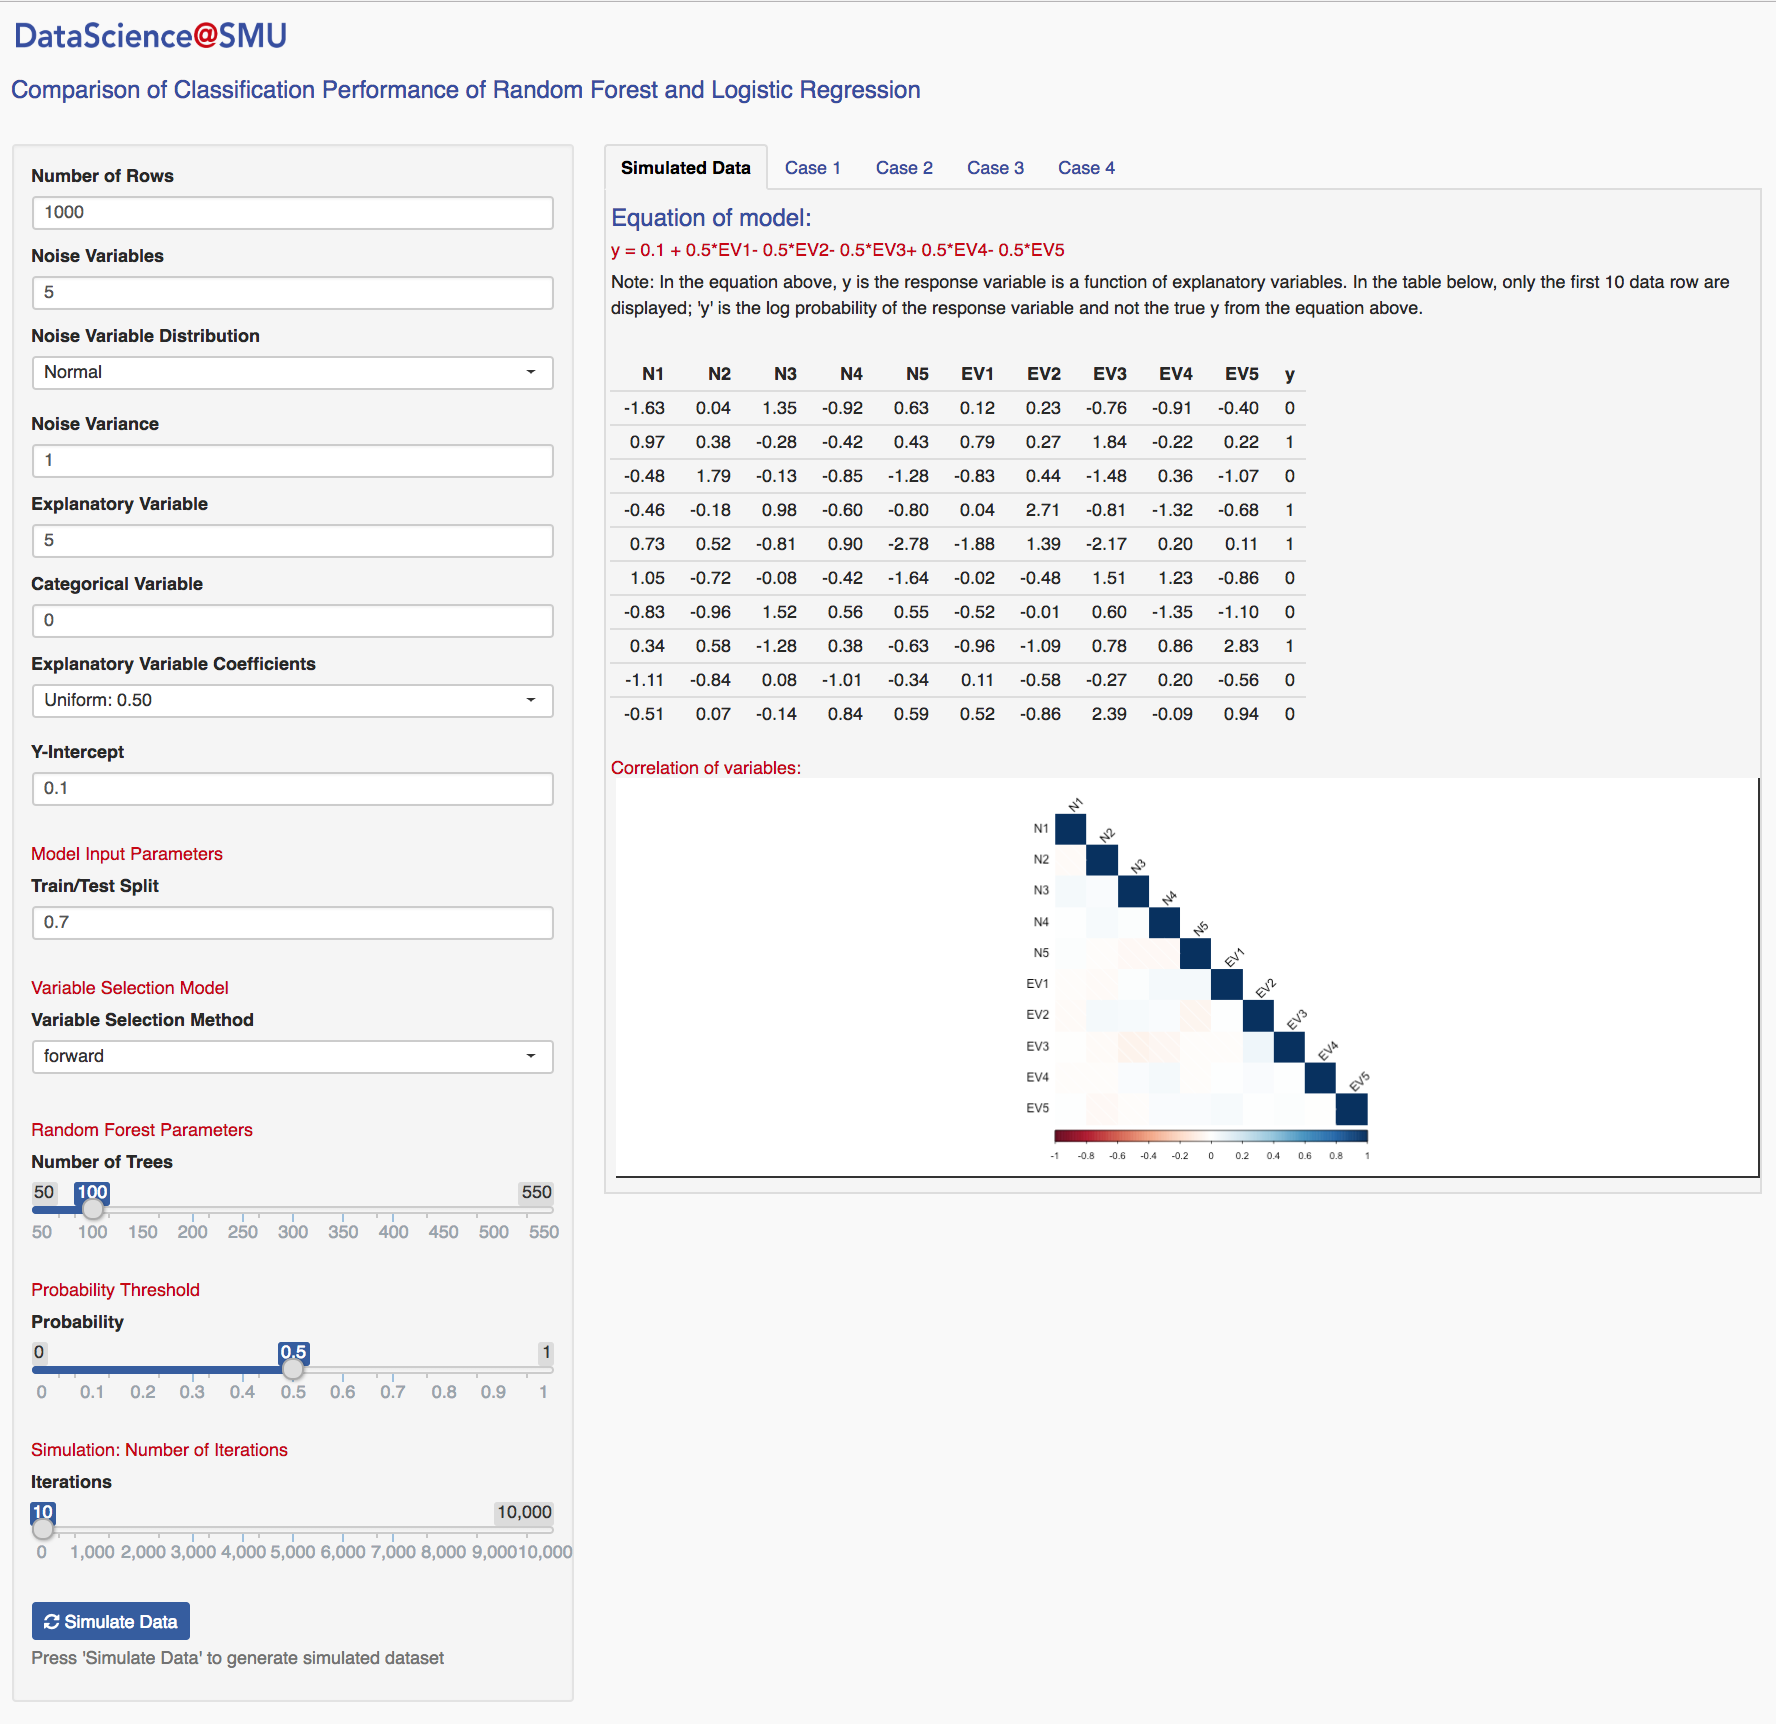
\includegraphics[width=0.95\textwidth]{full-tool.png}
\caption{Data Simulator}
\label{fig:rshiny}
\end{figure}


\noindent 
For performing numerical simulations, creating synthetic datasets is pivotal for the analysis. SimStudy is an open source package in the R programming language. This was leveraged in this work as the method for producing datasets of various structures. To compare model performance for binary classification, we needed a response variable, which we will call 'y', which is a function of only the explanatory variables 'x' included in the model equation (Eq. 1) and displayed in the tool in Figure~\ref{fig:dataset}.  Figure~\ref{fig:dataset} is a screenshot of the first tab in the center content of the tool.  It displays the equation as well as the first 10 rows of the dataset with all columns of 'EV', 'N', and the response 'y'. The explanatory variable 'EV' is related to the binary response, while the noise variables 'N' are not. The binary response variables take on the value of either a 1 or 0; thus the formula represents the log of odd which is the probability of the response being a 1 or 0. The parameter estimates explain the relationship between independent variables 'X' and the dependent variable 'Y', and the 'Y' scale is known as the logit, log of odds. For each simulation case study explored in the work, the default parameter estimate, beta, is set to a uniform 0.50 and the input features, both noise and explanatory variables, are all continuous and normally distributed. 

\begin{figure}
\centering
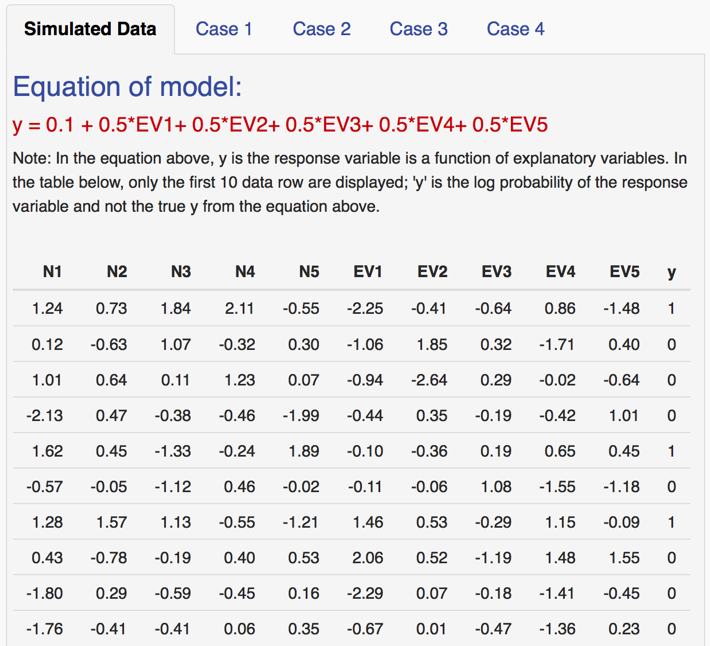
\includegraphics[scale=0.75]{dataset.png}
\caption{Equation of the response variable and first 10 rows of the simulated dataset}
\label{fig:dataset}
\end{figure}

\noindent 
The rest of the tabs in the tool are for the case studies that we explored in this work.  On each tab, there is a description of what each case is simulating and the results of running random forest and logistic regression predictions on the simulated data.  The average of the evaluation metrics are summarized in a table and line charts and a spread of the evaluation metrics are seen in a boxplot. Figure~\ref{fig:center} is an example of the summary, table of average evaluation metrics for each model, and a two sample t-test for the difference in models.

\begin{figure}
\centering
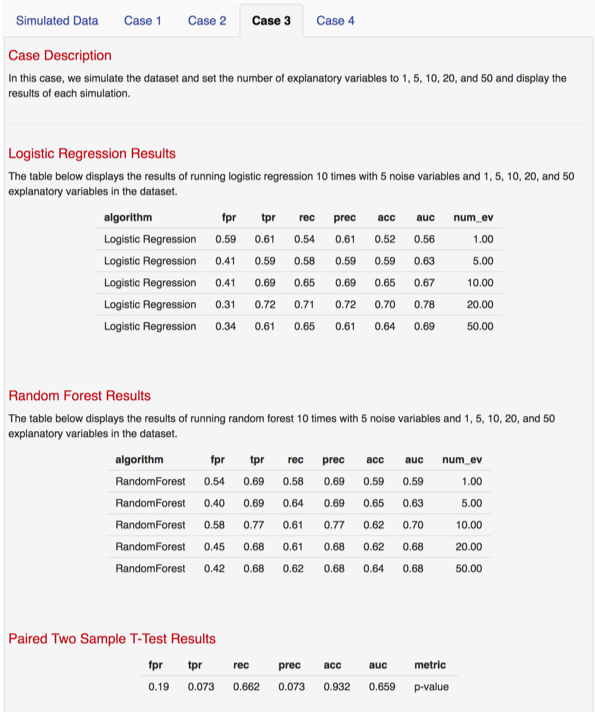
\includegraphics[scale=0.99]{center.png}
\caption{Example case study tab}
\label{fig:center}
\end{figure}


\section{Criteria for Model Comparison}
\noindent 
When comparing overall model performance, accuracy, true positive rate, false positive rate, precision, recall, and AUC were considered as the core metrics.  These are all classification and misclassification metrics.  Accuracy, true, and false positive rates are classic classification metrics while precision, recall, and AUC are functions of true and false positive rates.

\begin{table}[]
\begin{tabular}{|l|l|}
\hline
Accuracy                   & (TP + TN) / (TP + TN + FP + FN)      \\ \hline
True Positive Rate (TPR)   & TP / (TP + FN)                       \\ \hline
False Positive Rate (FPR)  & FP / (FP + TN)                       \\ \hline
Precision                  & TP / (TP + FP)                       \\ \hline
Recall                     & TP / (TP + FN)                       \\ \hline
Area Under the Curve (AUC) & Integral area of plotting TPR vs FPR \\ \hline
\end{tabular}
\caption{Evaluation metrics for comparison of model performance}
\label{eval_metrics}
\end{table}

\noindent 
Our work consists of four different simulation cases.  Each simulation case uses what the user entered on the left side to generate the dataset but also takes one characteristic and varies it while keeping all else constant. For cases 1 through 3 we used 1000 as the number of observations while case 4 looked at model performance with respect to changes in the number of observations. 

\noindent 
For each simulation case, the dataset was randomly partitioned into 70\% being utilized to train the model while the remainder 30\% is left out of training the model and used to test the model. To determine how well a model predicts on the training data, we used a few different metrics. The first metric is accuracy, which is the percentage of correct classification. If the data point is actually a success, how often does the model predict success and if it was a failure, how often is a failure predicted. Accuracy is a nice overall average of how well a model can predict and simple to compute.  However, if there is a class imbalance meaning 99\% of my data is a success and only 1\% of the time it is a failure, the model could predict success 100\% of the time and have a very high accuracy of 99\%.  This causes an illusion that a model is performing very well but when implemented and used in the real world it may not be useful. In cases where there is a large class imbalance we may want to look at other evaluation metricssuch as true positive rate and false positive rate.  


\noindent 
True positive rate, also known as sensitivity, is calculated as the portion of positives or successes that are correctly identified. On the other hand, false positive rate is the portion that was incorrectly identified as positive or success but is actually negative (Pedregosa et al). Depending on the application and domain, one may care about incorrectly classifying a positive more than incorrectly classifying a negative.  For example, when dealing with anything medical or health related, such as predicting if a patient will have dementia, it is extremely important to have a low false positive rate because telling someone they have dementia when they do not can cause a lot of emotional stress amongst other issues.  False positive rate is also important when determining quality where the cost of a misclassification is high.  For instance, to test a silicon wafer for defects, a machine goes through and returns a report with an outline of a wafer and places a dot on the area of the wafer where there could be a defect in the material or conductivity.  If there are too many defects, a tester will often throw away out the entire wafer.  However, one wafer could cost upwards of \$10,000 so throwing away a wafer that could be perfectly fine because of a false defect can be very costly mistake.  When dealing with an automated event or airport security, it may be okay to have a higher false negative rate because it is a relatively cheap and non-life-threatening task to confirm an automated alert as actually positive.


\noindent 
After running the simulated dataset through each model, the results can be graphically represented using the receiver operating characteristic curve or ROC curve as seen in Figure~\ref{fig:roc}.  The ROC curve is a graph with the x axis from 0 to 1 of the false positive rate, and the y axis from 0 to 1 of the true positive rate at various threshold settings.  A perfect predictor would have a false positive rate of 0 and a true positive rate of 1.  When graphed over a series of thresholds, the area under the curve (AUC) can provide a single value for providing insight into how well the model is classifying the labels. For interpretation, the higher the AUC, the better the model performs. The AUC is more descriptive than accuracy because it is a balance of accuracy and false positive rate.
\begin{figure}
\centering
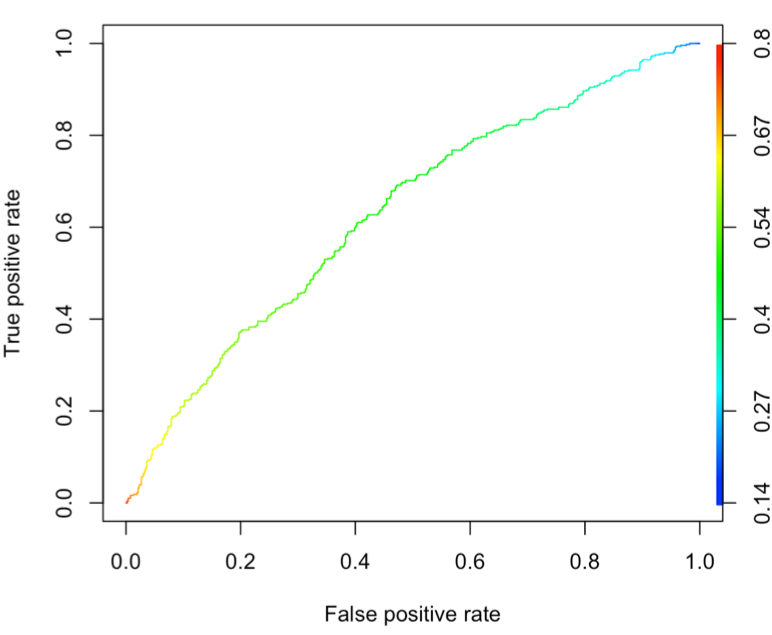
\includegraphics[scale=0.99]{roc.png}
\caption{Example ROC curve}
\label{fig:roc}
\end{figure}

\noindent 
Both recall and precision are often reported for classification performances.  Recall is the ability to find all relevant instances while precision is the proportion of the data points the model considers relevant that are actually relevant.  Precision is the number of true positives divided by the number of true positives and false positives.  This provides an indication of the ability of a classification model to identify only relevant data.  For example, if running a preliminary test to predict if a patient has a disease or not, precision would be equal to the number of patients who have the disease and were predicted correctly divided by the number of patients who have the disease and were predicted correctly plus the patients incorrectly predicted as having the disease.  Recall is the number of true positives divided by the number of true positives and false negatives. Recall tells us the ability of a model to find all relevant cases within a dataset.  Using the example above, recall would be equal to the number of patients who have the disease and were predicted correctly divided by the number of patients who have the disease and were predicted correctly plus the patients incorrectly predicted as not having the disease. Thus, a high recall is desired to find all patients who actually have the disease and can allow a lower precision if the cost of a follow up check is low.

\section{Analysis and Results}
\noindent 
The analytical tool has four case studies that runs on simulated data based on the user's customized inputs. Figure~\ref{fig:center-content} is an example of what the output of the results looks like.  On each tab of the tool, a table of the evaluation metrics for each model as well as line graphs of those evaluation metrics.  For accuracy, true and false positive rates, a boxplot is displayed of the spread of all values for each simulation run.  For example, if we set the number of simulations to 1000, the table and line chart will show me the average value of all 1000 simulations and the boxplots take into account the  values for each of the 1000 simulations.

\begin{figure}
\centering
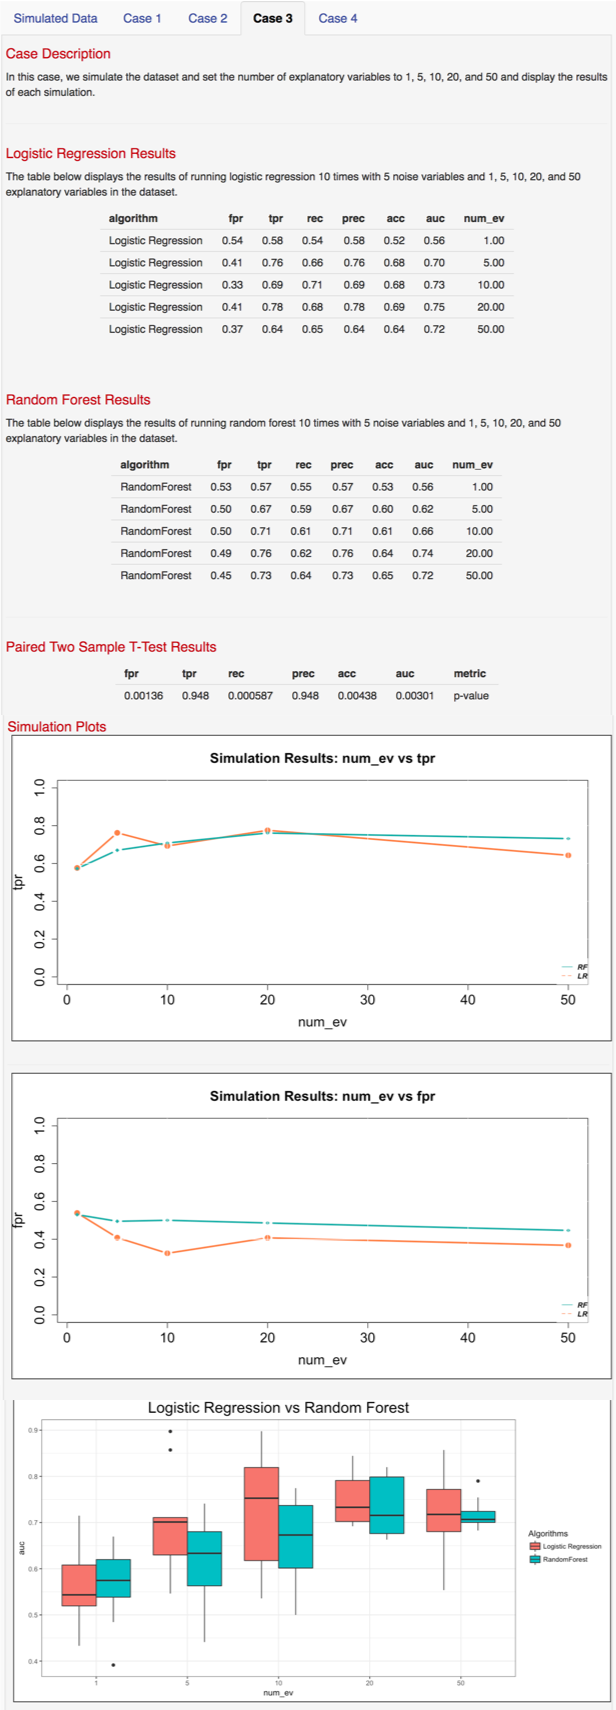
\includegraphics[scale=0.75]{results_long_2.png}
\caption{Results of running each model of simulated data in each case study}
\label{fig:center-content}
\end{figure}

\subsection{Case 1}
\noindent 
The first case investigated was comparing model performance with respect to change in variance in the explanatory and noise variables. The hypothesis was that an increase in variance would strengthen the accuracy for both models. For this simulation case, the application was configured to run 1000 simulations for 1000 observations. In the top row of Figure~\ref{fig:case1results}, the results display the accuracy for varying levels of variance in 10 noise and 5 explanatory variables. There is both visual evidence from Figure~\ref{fig:case1results} and statistical evidence  from the paired t test (p-value < .05) to suggest that, on average, the accuracy of the logistic regression model is  greater than that of the random forest model. 


\noindent 
The bottom row of Figure~\ref{fig:case1results} displays the results of the true positive rate on the left and false positive rate on the right. The true positive rate for both models are nearly the same at each variance level.  However, one can see that the false positive rate for random forest is not significantly higher than logistic regression (p-value = 0.63).  Even though both models have the same performance in terms of correctly classifying a true value as true, the false positive rate for random forest is higher than logistic regression.  This causes logistic regression to outperform random forest in terms of overall accuracy at each level of variance.

\begin{figure}
\centering
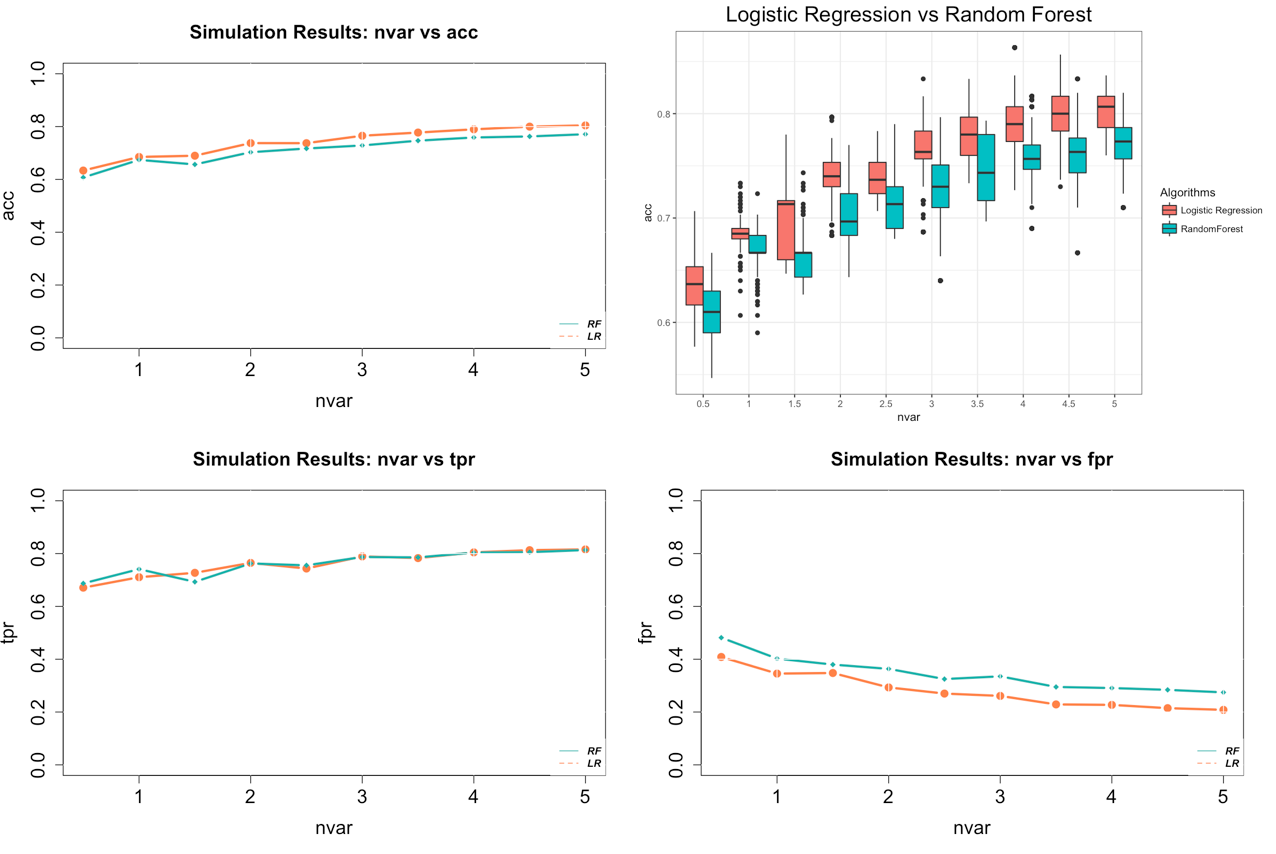
\includegraphics[scale=0.55]{case1.png}
\caption{Case 1 Simulation Results: 5 noise and 10 explanatory variables}
\label{fig:case1results}
\end{figure}
\noindent 
The simulation is conducted again, but now adding more noise variables (noise = 100) and the results of the accuracy is shown in the top row of Figure~\ref{fig:case1resultsb}. By looking at Figure~\ref{fig:case1results} and Figure~\ref{fig:case1resultsb}, a similar trend is observed. With a p-value less than 0.05, there is strong evidence to suggest that a significant difference in accuracy between the two models exists. The boxplots for this simulation is also comparable with 10 noise variables where minimal overlap in the boxplots for each model at each level of variance is observed. However, with 100 noise variables, the boxplots are much more consistent in that they are all about the same size for each level of variance.  In Figure~\ref{fig:case1resultsb}, the boxplots for each model are noticeably different sizes.


\noindent 
The bottom row of Figure~\ref{fig:case1resultsb} displays the true positive rate on the left and false positive rate on the right with 100 noise variables and 5 explanatory variables over increasing levels of variance in the variables. Interestingly, for variance 0.5 to 2.5 and a lot of noise, random forest has a higher true positive rate.  At around variance = 3.0 and higher, random forest still has a higher true positive rate, but it is not as large of a difference from logistic regression than variance < 2.5. The false positive rate for random forest is again higher than logistic regression so the gap in higher true positive rate is not enough to make overall accuracy higher for random forest.

\begin{figure}
\centering
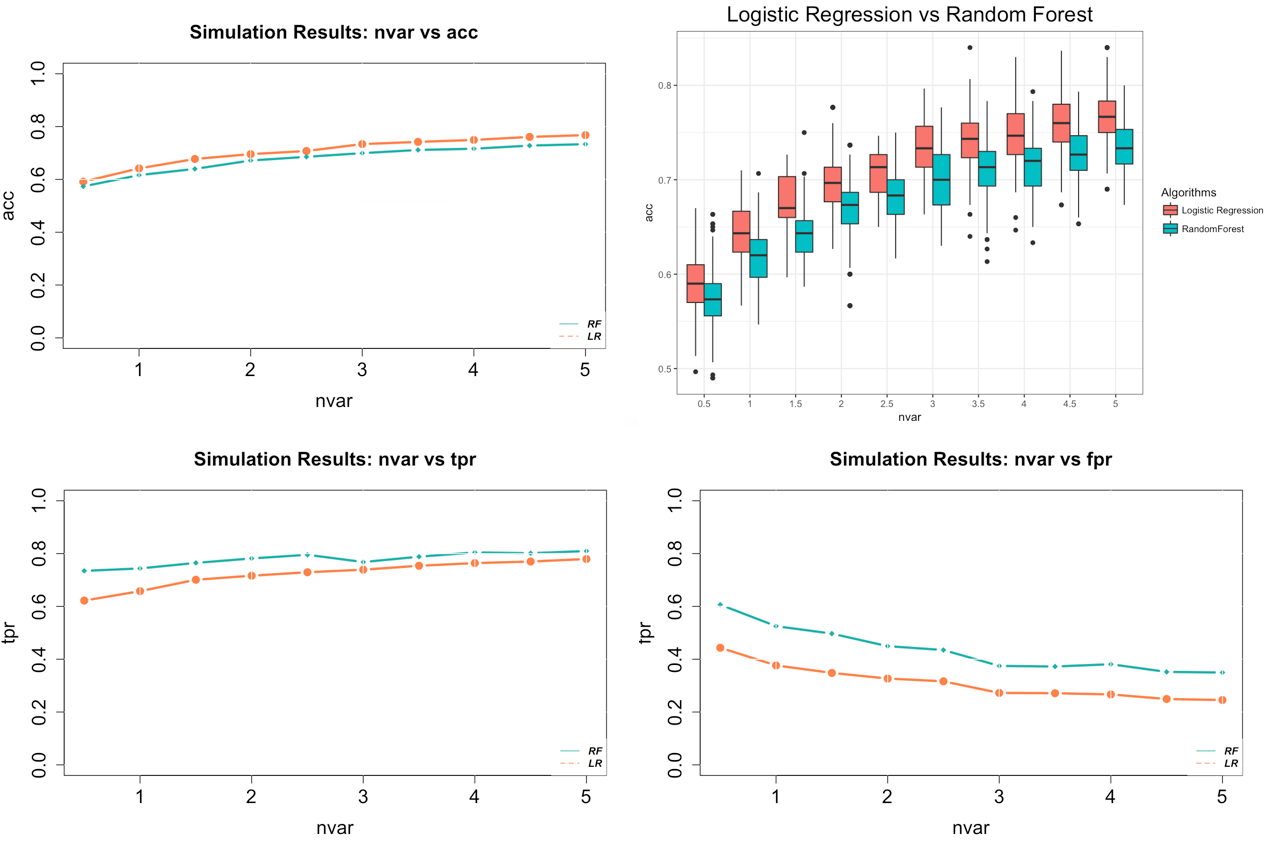
\includegraphics[scale=0.55]{case1_b.png}
\caption{Case 1 Simulation Results: 100 noise and 5 explanatory variables}
\label{fig:case1resultsb}
\end{figure}

\subsection{Case 2}
\noindent 
In case 2, we compared model performance with respect to change in the amount of noise in the dataset. We first did this by running 1000 simulations on a dataset with the number of noise variables = 1, 5, 10, 20, and 50.  In Figure~\ref{fig:case2results}, we see the results of the accuracy for each model when the number of explanatory variables is 5 with 1000 observations.  As we expected, as the amount of noise in the dataset increases, we see the accuracy start to decline for both models. However, we were not able to get the full picture by stopping at 50 noise variables, so we ran this again increasing the noise further.  Figure~\ref{fig:case2resultsb} shows the results of accuracy when setting the number of noise variables to 1, 5, 10, 20, 40, 60, 80, 100, 150, 200.  Accuracy is still slightly declining as we increase the noise past 50 noise variables and logistic regression is still performing with a higher accuracy (p-value = 9.559e-07).

\begin{figure}
\centering
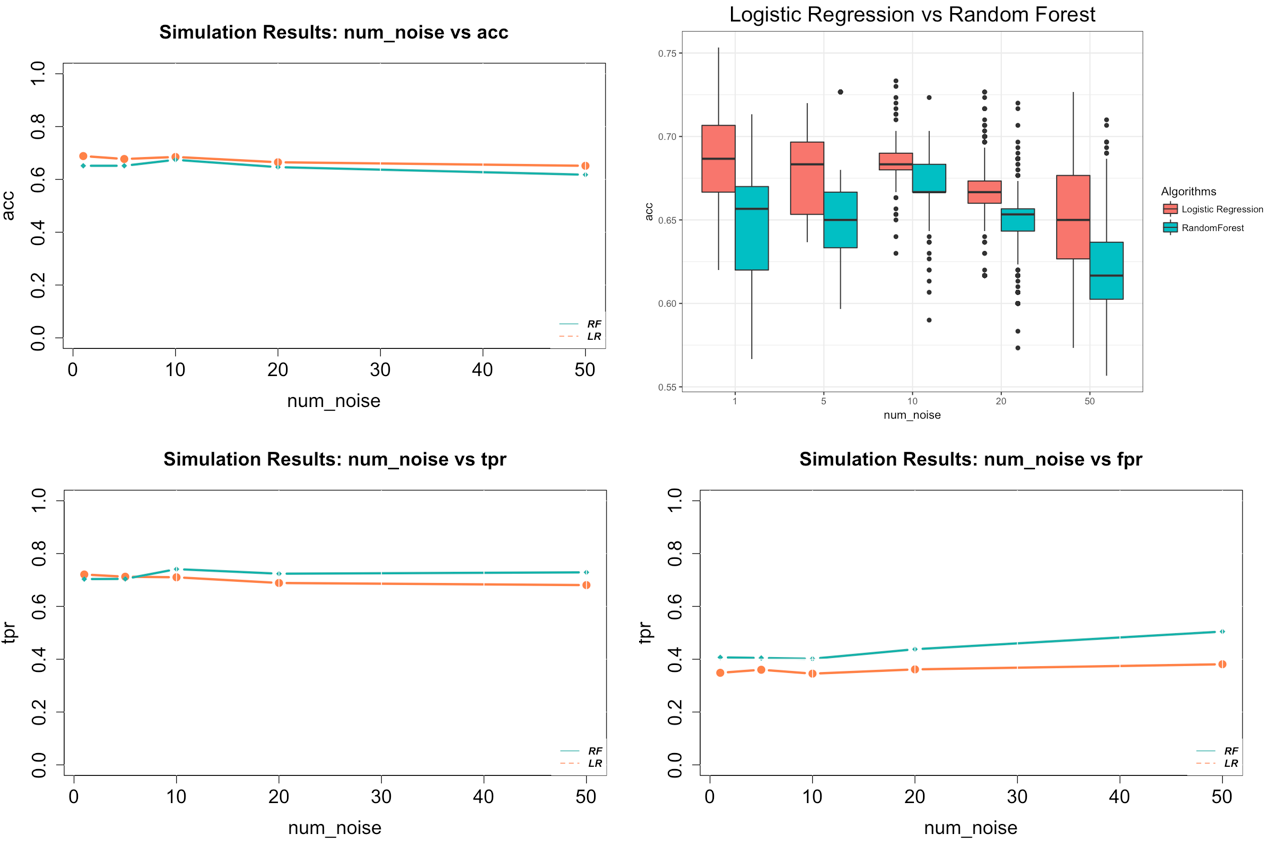
\includegraphics[scale=0.55]{case2.png}
\caption{Case 2 Simulation Results: 1 to 50 noise variables}
\label{fig:case2results}
\end{figure}

\noindent 
The bottom rows of Figures~\ref{fig:case2results} and ~\ref{fig:case2resultsb} show the true positive rate on the left and false positive rate on the right.  For true positive rate, when the number of noise variables is the less than or equal to the number of explanatory variables in the dataset, logistic regression is higher.  However, once the number of noise variables exceeds the number of explanatory variables, random forest begins to have a higher true positive rate than logistic regression.  As the amount of noise in the data increases, the false positive rate for both models also increase.  However, the rate of increase in false positive rate for random forest is greater than the rate of increase in false positive rate for logistic regression as noise increases.  Logistic regression does not have much change in true or false positive rate as noise increases past 50, but random forest false positive rate noticeably increases past 50 noise variables.

\begin{figure}
\centering
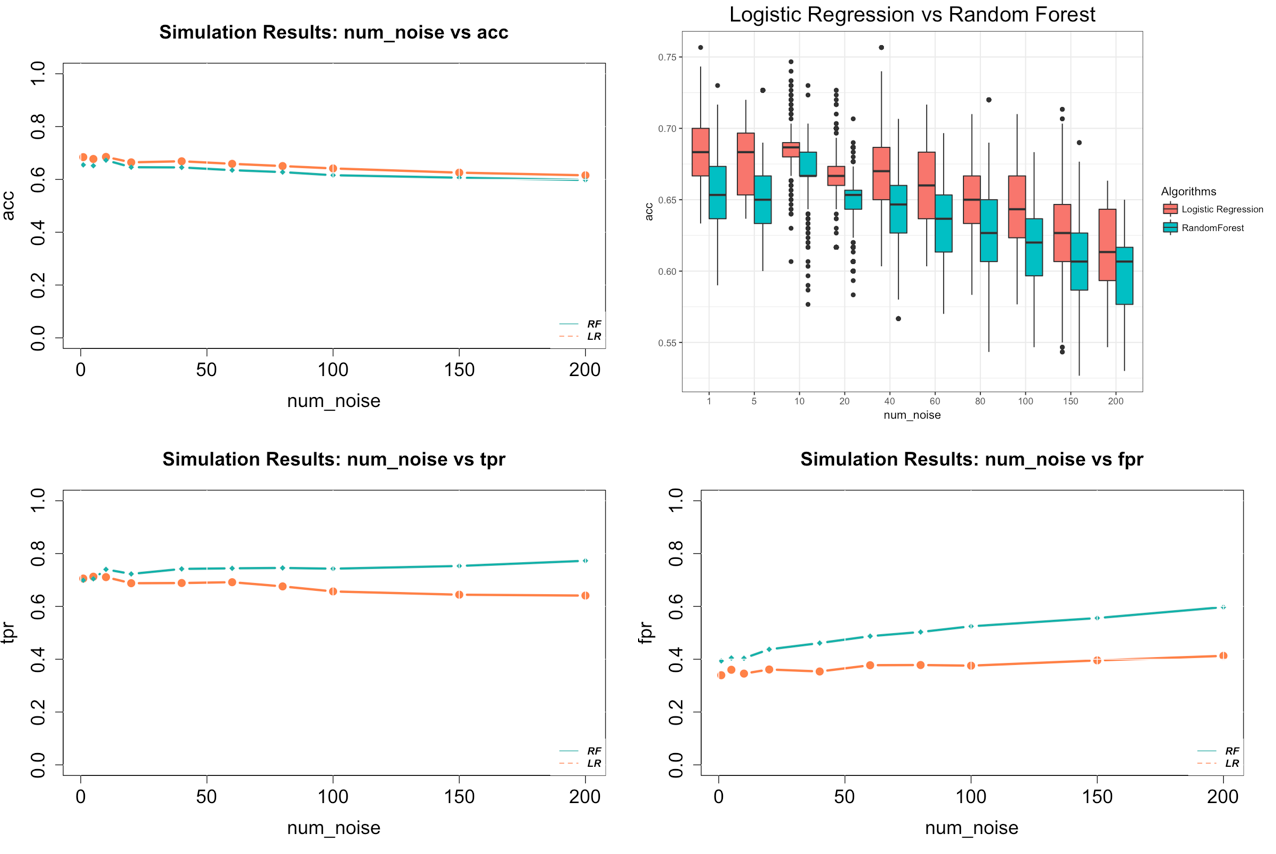
\includegraphics[scale=0.55]{case2_b.png}
\caption{Case 2 Simulation Results: 1 to 200 noise variables}
\label{fig:case2resultsb}
\end{figure}

\subsection{Case 3}
\noindent 
In case 3, we compared model performance with respect to change in the number of explanatory variables in the dataset.  In other words, the number of variables that relate to the response variable we are predicting. We did this by running 1000 simulations on a dataset with the number of explanatory variables = 1, 5, 10, 20, 30, 40, 50.  In the top row of Figure~\ref{fig:case3results}, we see the results of the accuracy for each model when the number of noise variables is 50 with 1000 observations.  With 30 or less explanatory variables, as the number of explanatory variables in the dataset increases, the accuracy increases as well.  When the number of explanatory variables is above 30, random forest begins to taper off whereas logistic regression continues to increase in overall accuracy. 

\begin{figure}
\centering
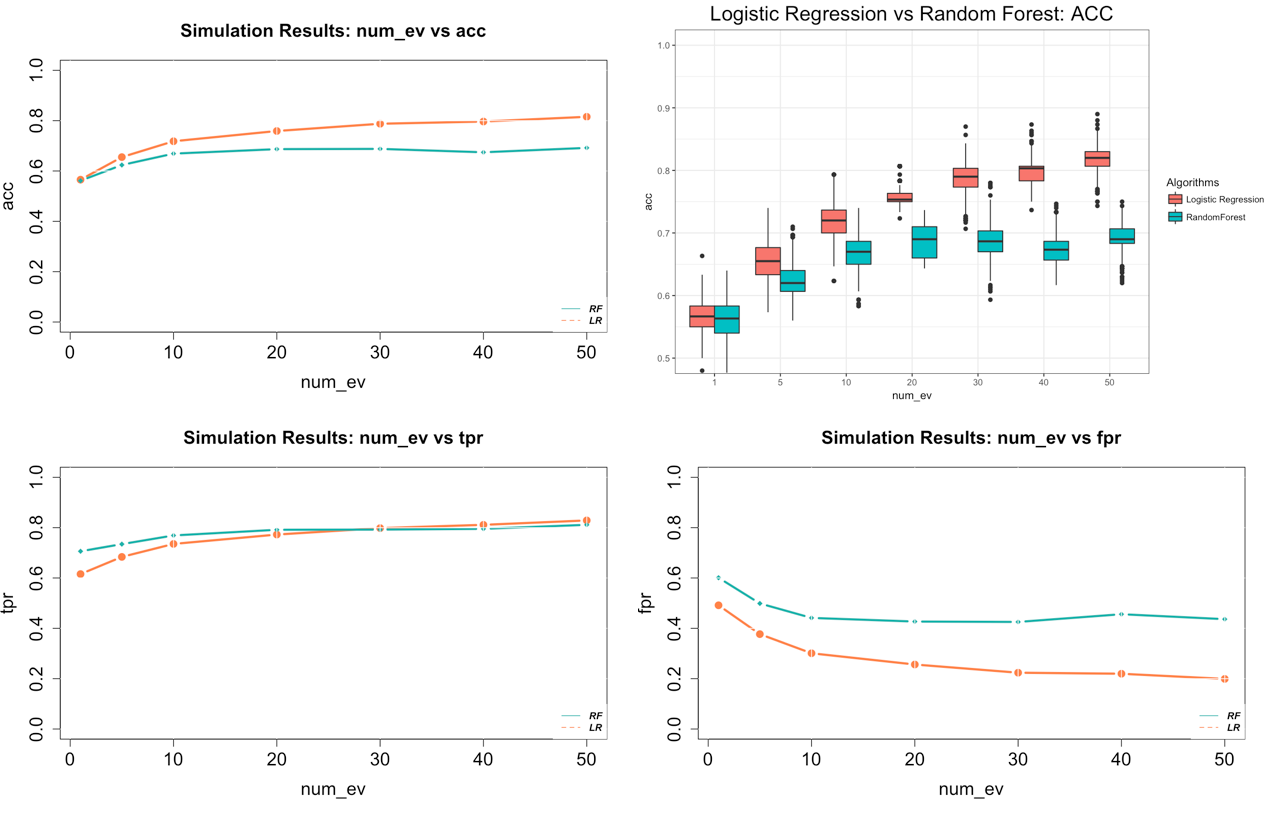
\includegraphics[scale=0.55]{case3.png}
\caption{Case 3 Simulation Results}
\label{fig:case3results}
\end{figure}

\noindent 
The bottom row of Figure~\ref{fig:case3results} displays the true positive rate on the left and false positive rate on the right.  When we look at the true positive rate for the models, below 30 explanatory variables, random forest had a higher true positive rate.  At 30 explanatory variables, logistic regression crosses over and continually increases to have a higher true positive rate than random forest.  When we look at false positive rate, logistic regression decreases as we add more explanatory variables.  Random forest false positive rate initially decreases from 1 to 10 explanatory variables but from 10 to 50 explanatory variables, there is not much change.  The crossover point in true positive rate at 30 explanatory variables and the continued decrease in false positive rate for logistic regression as explanatory variables increases is evident in the overall accuracy plots.  From the accuracy plots, we can see the drastic gap in performance of the two models after 20 to 30 explanatory variables.


\subsection{Case 4}
\noindent 
This simulation case study looked at iteratively increasing the number of observations in the dataset from 10 to 10000 while holding the number of explanatory variables in the model constant. A total of four different subcases were evaluated in which the number of explanatory variables ranged from 1,10,20, and 50; each case comprised of 10 noise variables. Given the computational complexities and completion time to train and validate a model for 1000 simulation as described in the previous cases and increasing the overall size of the dataset, the total number of simulations for specific case study is 10. Hence the moderate variance observed in Figure~\ref{fig:case4_acc_results} and Figure~\ref{fig:case4_tpr_results}. 

\begin{figure}
\centering
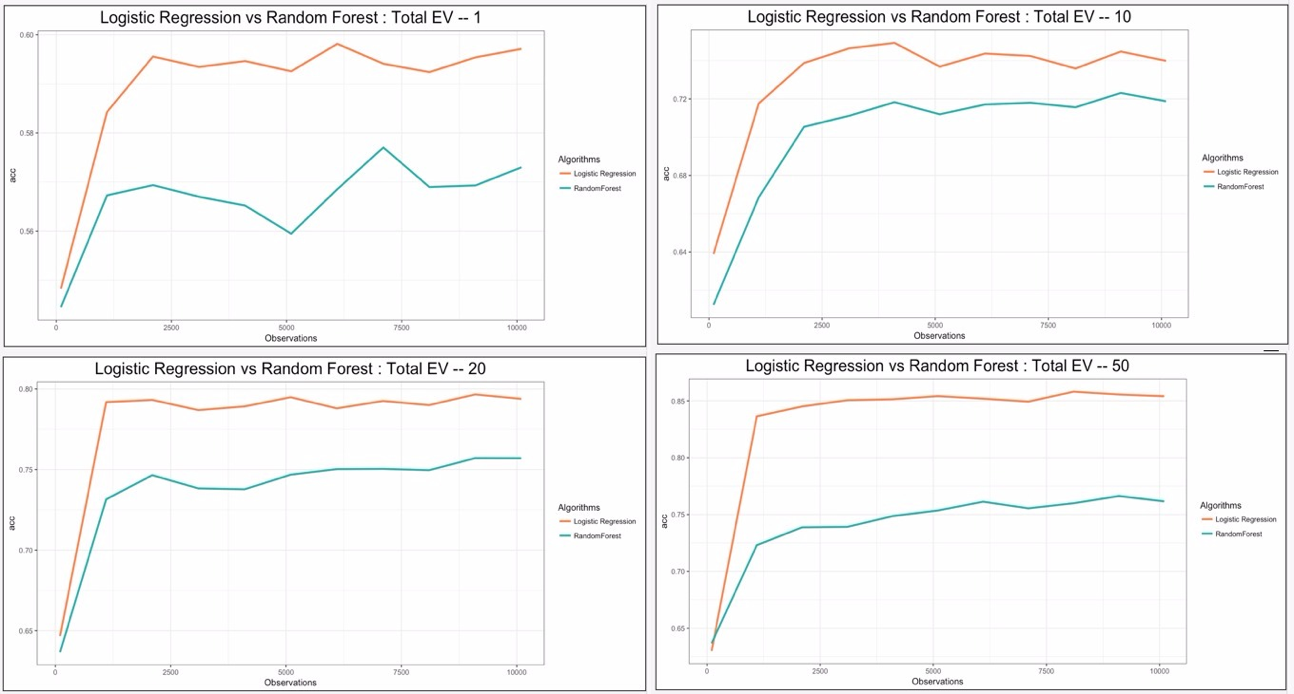
\includegraphics[scale=0.55]{case4_acc.png}
\caption{Case 4 Simulation Results - Accuracy}
\label{fig:case4_acc_results}
\end{figure}

\begin{figure}
\centering
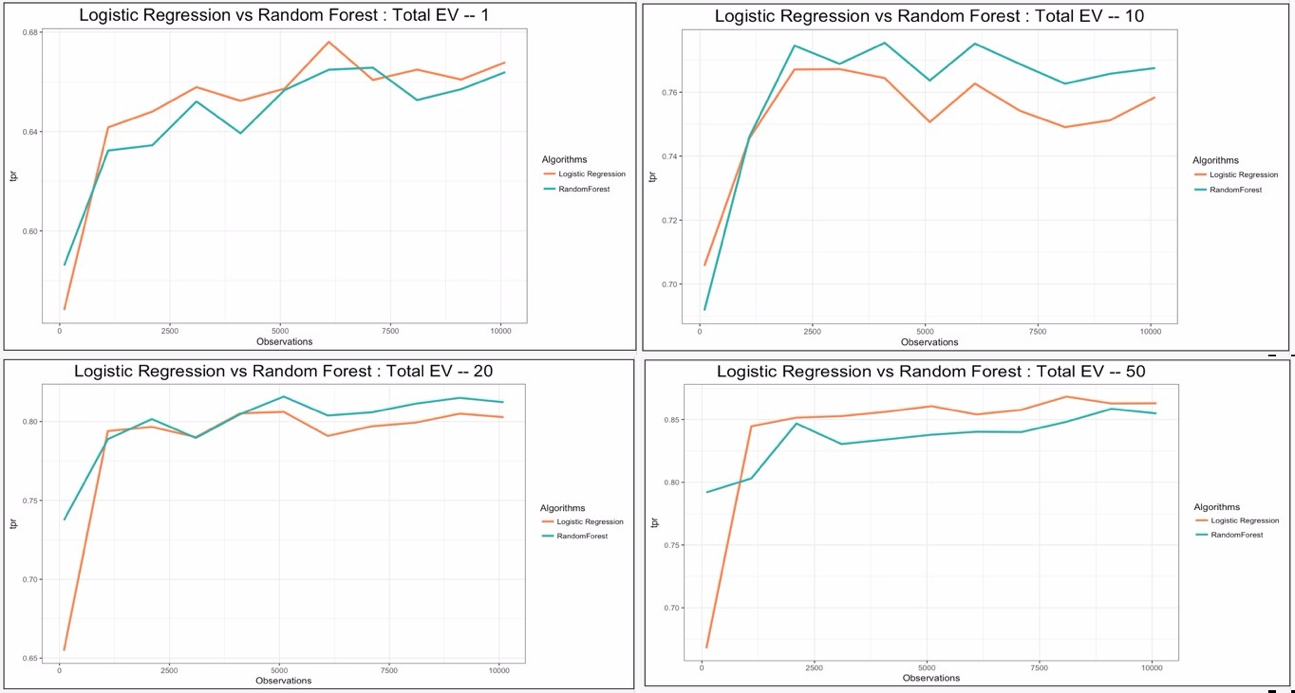
\includegraphics[scale=0.55]{case4_tpr.png}
\caption{Case 4 Simulation Results - True Postive Rate}
\label{fig:case4_tpr_results}
\end{figure}


\noindent 
One of the interesting findings in this simulation case is random forest and logistic regression perform nearly the same up until approximately 1000 observations in the dataset before diverging or in some instances crossing over as shown in Figure~\ref{fig:case4_tpr_results}. Secondly, in Figure~\ref{fig:case4_acc_results}, the overall accuracy for logistic regression is consistently higher than random forest with 100 trees as both the number of explanatory and observations increases. With 10 and 20 explanatory variables included in the model respectively, the difference in overall accuracy is at a minimal compared to the case where 50 explanatory variables are included. 


\noindent 
Additional analysis will need to be performed to determine if these observations are consistent when random forest is trained with a larger number of trees in addition to increasing the number of simulations to have a better understanding of the true accuracies.

\subsection{Summary of Results}
\noindent 
In summary, we found that when increasing the variance in the explanatory and noise variables, logistic regression consistently performed with a higher overall accuracy as compared to random forest. However, the true positive rate for random forest was higher than logistic regression and yielded a higher false positive rate for dataset with increasing noise variables. In all simulated case studies, we consistently found that the false positive rate for random forest with 100 trees was statistically different than logistic regression. In general, logistic regression performs better when the number of noise variables is less than or equal to the number of explanatory variables and random forest has a higher true and false positive rate as the number of explanatory variables increases in a dataset.  Logistic regression and random forest are comparable for smaller datasets with less than 1000 observations.


\section{Ethics}
\noindent 
Data science is a rapidly evolving field and along with it's success comes data privacy concerns. With massive amounts of data being collected today more so than ever before, our professional requirement is to conduct responsible and ethical innovation. In doing so, adhering to such ethical practices can continue fostering progress in data science and protect individual and group rights \cite{floridi}. Our data is synthetically generated via the analytical tool developed for our analysis. Therefore, there is no liable concerns of the availability, integrity, usability, and security of the data. We do not have functionality that will allow users to upload their own dataset to this tool and run an evaluation so we do not store any of the users data. Because data is not currently being stored, security scans will not be performed on the application, but we applied best practices to avoid any known security vulnerabilities. If any issues are reported we will also notify users of potential deficiencies as well as correct these deficiencies if possible. Finally, in the context of the synthetic data generated in the application, there is no legal violations or security concerns.  Our tool should be used for education and simulation purposes only and is a simple calculation tool.  Our tool does not suggest one model over another, the tool will only calculate and display the results.  Because of this, we allow the users to make their own decisions on which model is best for their circumstances. 


\section{Conclusions}
\noindent 
We are waiting to add hard conclusions here.  Unfortunately, our results are based off of running random forest set at 100 decision trees.  In the next five weeks we will re-run simulations are come to conclusions.



\section{Future Work}
\noindent 


\newpage
\begin{thebibliography}{18}

\bibitem{couronne}
Couronné, Raphael. Probst, Philipp.Boulesteix, Anne-Laure. Random forest versus logistic regression: a large-scale benchmark experiment. BMC Bioinformatics. 2018

\bibitem{erdem} 
Beğenilmiş, Erdem; Üsküdarlı, Suzan.  Organized Behavior Classification of Tweet Sets using Supervised Learning Methods. eprint arXiv:1711.10720. 11/2017.

\bibitem{bertrand} 
Bertrand Michel. A Statistical Approach to Topological Data Analysis. Statistics [math.ST]. UPMC Université Paris VI, 2015.

\bibitem{breiman} 
Breiman, L. Random Forests. 2001

\bibitem{floridi} 
Floridi L, Taddeo M.  What is data ethics? Phil.Trans.R.Soc.A 373: 20160360. 2016

\bibitem{chazal} 
Frédéric Chazal; Bertrand MichelAn introduction to Topological Data Analysis: fundamental and practical aspects for data scientists. 2017

\bibitem{goodfellow} 
Goodfellow, Ian; Bengio,Yoshua; Courville, Aaron. Deep Learning. MIT Press. 2016

\bibitem{graham} 
Graham, Dunn. Regression Models for Method Comparison Data. Journal of Biopharmaceutical Statistics 17:4, pages 739-756. 2007

\bibitem{guerreiro} 
Guerreiro, Manuela; Maroco, João; de Mendonça, Alexandre; Rodrigues, Ana; Santana, Isabel; Silva, Dina. Data mining methods in the prediction of Dementia: A real-data comparison of the accuracy, sensitivity and specificity of linear discriminant analysis, logistic regression, neural networks, support vector machines, classification trees and random forests. BMC Research Notes20114:299. https://doi.org/10.1186/1756-0500-4-299.

\bibitem{hastie} 
Hastie, T., Tibshirani, R., Friedman, J. The elements of statistical learning: data mining, inference and prediction. Springer. 2009

\bibitem{olson} 
Olson, Randal S.; Moore, Jason H.  Identifying and Harnessing the Building Blocks of Machine Learning Pipelines for Sensible Initialization of a Data Science Automation Tool. eprint arXiv:1607.08878. 07/2016. 

\bibitem{ng} 
Ng, Andrew. CS229 Lecture Notes. Stanford University. 2012

\bibitem{munch} 
Munch, Elizabeth. A User’s Guide to Topological Data Analysis. University at Albany. 2017

\bibitem{ruiz} 
Ruiz-Gazen, Anne; Villa, Nathalie Storms Prediction: Logistic Regression vs Random Forest for Unbalanced Data.

\bibitem{pedregosa} 
Pedregosa et al., Scikit-learn: Machine Learning in Python, JMLR 12, pp. 2825-2830, 2011.

\bibitem{thanh} 
Thanh Lam, Hoang; Thiebaut, Johann-Michael; Sinn, Mathieu; Chen, Bei; Mai, Tiep; Alkan, Oznur.  One button machine for automating feature engineering in relational databases. eprint arXiv:1706.00327. 06/2017.

\bibitem{wolper}
Wolper, D.H. "No free lunch theorems for optimization," in IEEE Transactions on Evolutionary Computation, vol. 1, no. 1, pp. 67-82, April 1997. doi: 10.1109/4235.585893

\bibitem{zoran} 
Zoran Bursac, C Heath Gauss, David Keith Williams, David W Hosmer: Purposeful Selection of Variables in Logistic Regression. Source Code for Biology and Medicine. 2008

\end{thebibliography}

\end{document}


